\part{ТЕХНОЛОГИЧЕСКИЙ РАЗДЕЛ}

\subsection{Модули для GPS микросхемы MAX2769}


\subsubsection{Serial-интерфейс}

\begin{figure}[h]
\center{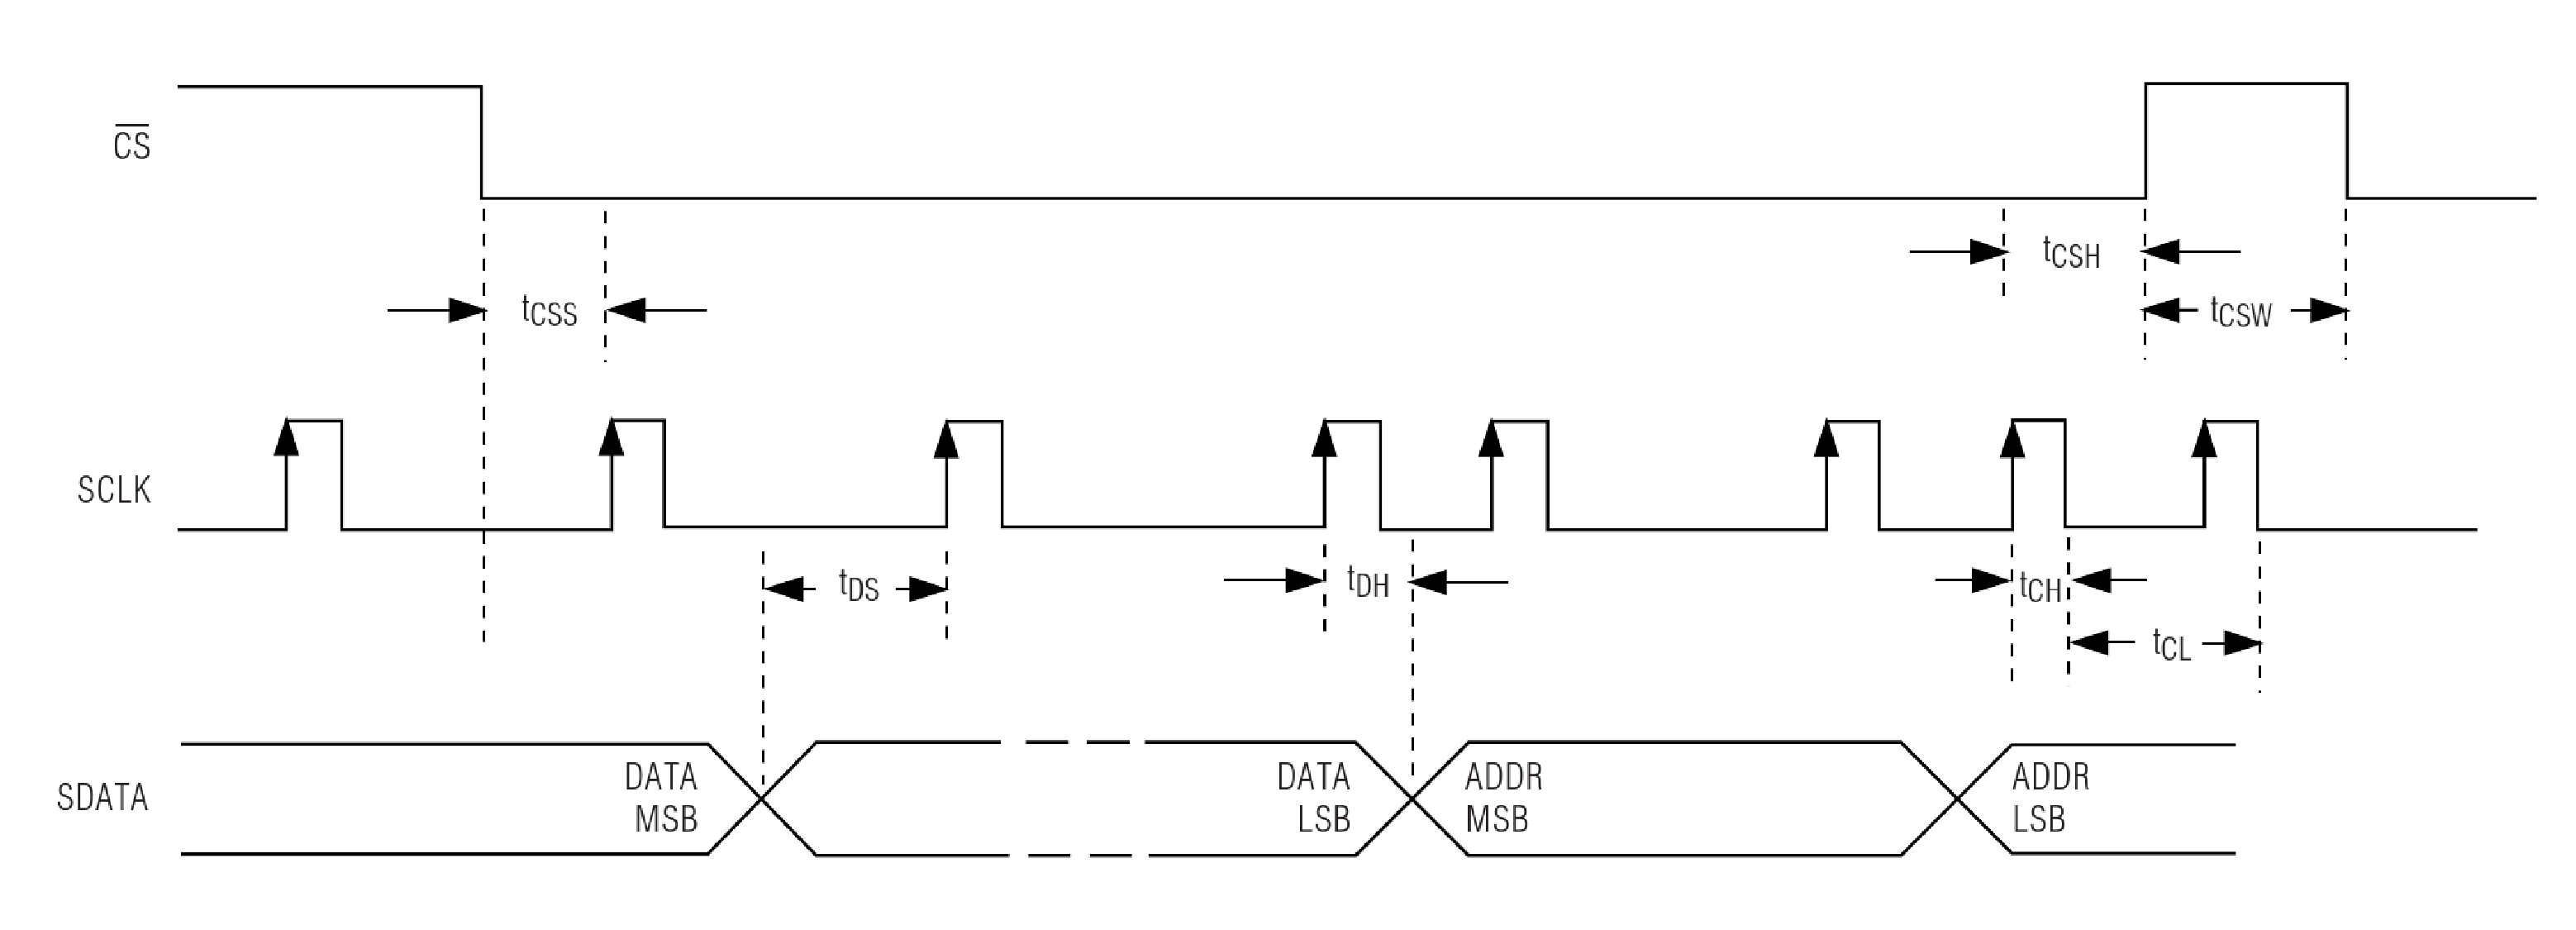
\includegraphics[width=1\linewidth]{./pics/gps_serial_times.eps}}
\caption{Временная диарамма serial-интерфейса GPS}
\end{figure}

\begin{table}[h]
\caption{Таблица 1. Временные требования для serial-интерфейса}
\label{tabular:serial-time}
\begin{tabular}{|c|p{250pt}|c|p{70pt}|}
 \hline  
  Символ & Параметр & Значение & Единица измерения  \\  
 \hline  
  $t_{css}$  & Время между падающим фронтом сигнала $\bar {CS}$ и передним фронтом сигнала SCLK	& 10 & нс  \\  
 \hline  
  $t_{ds}$   & Время установки данных на serial-линию	& 10 & нс \\  
 \hline  
  $t_{dh}$   & Время удержания данных на serial-линии	& 10 & нс \\  
 \hline  
  $t_{ch}$   & Время нахождения Сlock-сигнала serial-интерфейса в состоянии 1 & 25 & нс \\  
 \hline  
  $t_{cl}$   & Время нахождения Сlock-сигнала serial-интерфейса в состоянии 0 & 25 & нс \\  
 \hline  
  $t_{csh}$  & Время между крайним возрастающим фронтом сигнала SCLK и падающим фронтом сигнала $\bar {CS}$ & 10 & нс \\  
 \hline  
  $t_{csw}$  & Время $\bar {CS}$ в активном состоянии    & 1 & такт \\  
 \hline  
\end{tabular}
\end{table}

\begin{figure}[h]
\center{\includegraphics[width=1\linewidth]{./pics/gps_serial_clock_oscylloscope.eps}}
\caption{Clock-сигнал для serial-интерфейса GPS}
\end{figure}

\newpage
